\begin{task}{202}
В чемпионате хоккейной лиги расписание регулярного чемпионата составляется по следующему правилу: не обязательно каждый клуб играет со всеми другими, но среди любых трёх клубов хотя бы два из них должны сыграть матч между собой и никакая пара клубов не играет друг с другом больше одного раза. Всего в лиге играют $26$ клубов. Верно ли, что, как бы ни было составлено расписание, найдётся семь клубов, каждые два из которых играли матч друг с другом?
\end{task}

\begin{solution}
Рассмотрим неориентированный граф, с вершинами, в которых находятся клубы, и ребрами, которые существуют между двумя вершинами, если клубы, соответствующие этим вершинам, играли.\par
Среди любых трех клубов найдутся два, которые играли друг с другом, значит в графе не будет независимых множеств на трех и более вершинах.
\begin{enumerate}
\item Оценим $R(7, 3)$, используя свойства чисел Рамсея:
\[R(7, 3) \leq R(7, 2) + R(6, 3) = 7 + R(6, 3).\]

\item Оценим $R(6, 3)$, используя свойства чисел Рамсея:
\[R(6, 3) \leq R(6, 2) + R(5, 3) - 1 = 6 + R(5, 3) - 1 = 5 + R(5, 3).\]
Тут также предположили, что $R(5, 3)$ --- четное. Докажем это далее. 

\item Оценим $R(5, 3)$, используя свойства чисел Рамсея:
\begin{gather*}
R(5, 3) \leq R(5, 2) + R(4, 3) = 5 + R(4, 3);\\
R(5, 3) \leq 5 + R(4, 2) + R(3, 3) - 1 = 5 + 4 + 6 - 1 = 14;\\
R(5, 3) \leq 14.
\end{gather*}

\item Приведем пример, который покажет, что $14 \leq R(5, 3)$.
Для этого, построим два графа на $13$ вершинах: без независимых множеств размера $5$ и без клик размера $3$ соответственно.
\begin{figure}[H]
  \centering
  \begin{subfigure}[a]{0.24\linewidth}
    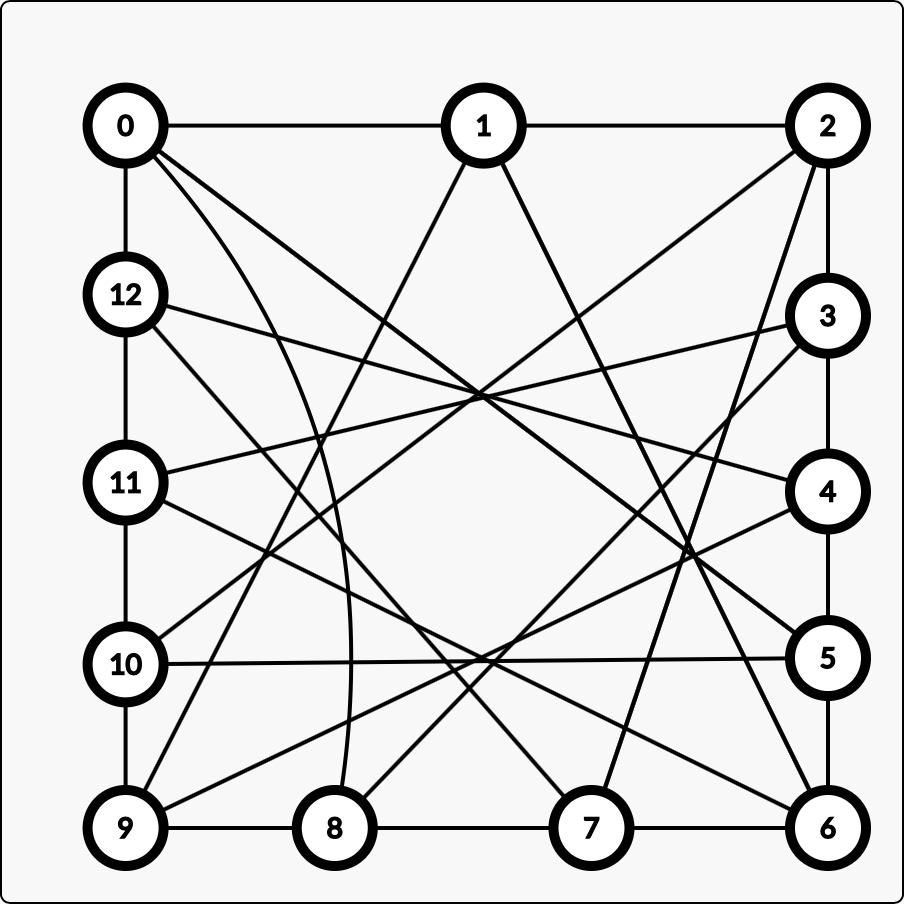
\includegraphics[width=\linewidth]{_img/202/01.png}
  \end{subfigure}
  \caption{граф без независимых множеств из пяти вершин.}
\end{figure}
\begin{figure}[H]
  \centering
  \begin{subfigure}[a]{0.24\linewidth}
    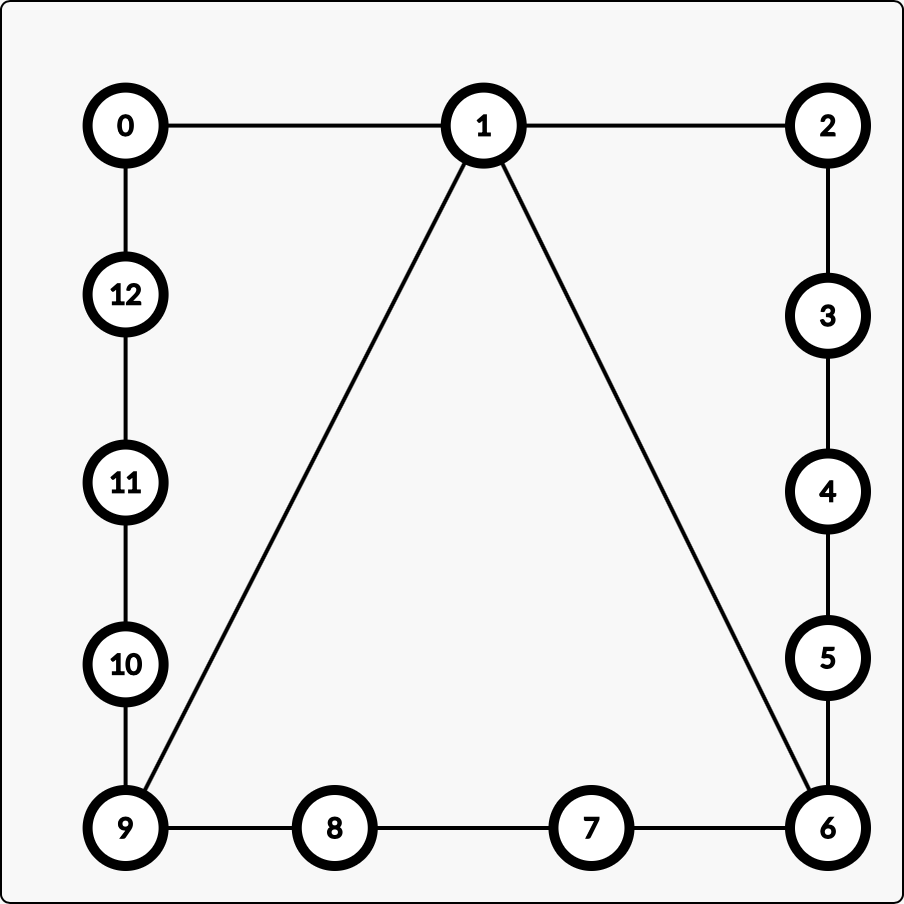
\includegraphics[width=\linewidth]{_img/202/02.png}
  \end{subfigure}
  \caption{граф без клик из трех вершин}
\end{figure}

\item
Получается, что
\begin{gather*}
    R(5, 3) = 14;\\
    R(6, 3) \leq 19;\\
    R(7, 3) \leq 26.
\end{gather*}
\end{enumerate}
Значит, в графе на $26$ вершинах найдется либо независимое множество размера $3$, либо клика размера $7$. По условию, независимых множеств размера $3$ в графе нет. Значит, среди каких-то семи команд каждые две играли между собой.
\end{solution}